% Copyright 2016 by Wang Kunzhen <wangkunzhen1993@gmail.com>.
%
% This is a latex template adapted from Till Tantau's Beamer template.
% It adds theme customizations for the convenience of users from the
% National University of Singapore. 
% 
% In principle, this file can be redistributed and/or modified under
% the terms of the GNU Public License, version 2.
%
% However, this file is supposed to be a template to be modified
% for your own needs. For this reason, if you use this file as a
% template and not specifically distribute it as part of a another
% package/program, I grant the extra permission to freely copy and
% modify this file as you see fit and even to delete this copyright
% notice. 

\documentclass[xcolor=dvipsnames]{beamer}





% There are many different themes available for Beamer. A comprehensive
% list with examples is given here:
% http://deic.uab.es/~iblanes/beamer_gallery/index_by_theme.html
% You can uncomment the themes below if you would like to use a different
% one:
% \usetheme{AnnArbor}
%\usetheme{Antibes}
% \usetheme{Bergen}
% \usetheme{Berkeley}
%\usetheme{Berlin}
%\usetheme{Boadilla}
% \usetheme{boxes}
%\usetheme{CambridgeUS}
%\usetheme{Copenhagen}
%\usetheme{Darmstadt}
%\usetheme{default}
%\usetheme{Frankfurt}
%\usetheme{Goettingen}
% \usetheme{Hannover}
% \usetheme{Ilmenau}
% \usetheme{JuanLesPins}
% \usetheme{Luebeck}
% \usetheme{Madrid}
\usetheme{Malmoe}
%\usetheme{Marburg}
% \usetheme{Montpellier}
% \usetheme{PaloAlto}
% \usetheme{Pittsburgh}
% \usetheme{Rochester}
% \usetheme{Singapore}
% \usetheme{Szeged}
% \usetheme{Warsaw}

\definecolor{nus-orange}{RGB}{239,124,0} 
\definecolor{nus-white}{RGB}{255,255,255}
\definecolor{nus-blue}{RGB}{0,61,124}
\definecolor{nus-black}{RGB}{0,0,0}

% Uncomment this section if you want the title background for each slide to be gradient like decaying from nus-orange to nus-white.
% \useoutertheme{sidebar}
% \usepackage{tikz}
% \usetikzlibrary{shadings}
% \colorlet{titleleft}{nus-orange}
% \colorlet{titleright}{nus-orange!45!nus-white}
% \makeatletter
% \pgfdeclarehorizontalshading[titleleft,titleright]{beamer@frametitleshade}{\paperheight}{%
%   color(0pt)=(titleleft);
%   color(\paperwidth)=(titleright)}
% \makeatother
% End of gradient slide title effect.

\setbeamercolor{section in head/foot}{bg=nus-blue, fg=nus-white}
\setbeamercolor{subsection in head/foot}{bg=nus-blue, fg=nus-white}
\setbeamercolor{frametitle}{bg=nus-orange, fg=nus-black}
\setbeamercolor{title}{bg=nus-orange, fg=nus-white}
\setbeamercolor{alerted text}{fg=nus-orange}
\setbeamercolor{block title}{fg=nus-blue}
\setbeamercolor{block body}{fg=nus-black}


% \useoutertheme[width=3\baselineskip,lef]{sidebar}
% \setbeamercolor{section in sidebar shaded}{fg=nus-blue, fg=nus-white}
% \setbeamercolor{structure}{fg=nus-blue}
% \setbeamercolor{navigation symbols dimmed}{fg=red!80!black}
% \setbeamercolor{navigation symbols}{fg=red!80!black}
% \setbeamercolor{navigation symbols}{bg=nus-blue}

\setbeamertemplate{theorems}[numbered]
\setbeamertemplate{propositions}[numbered]

\setbeamertemplate{bibliography item}{\insertbiblabel}
% \setbeamertemplate{bibliography item}[text]

\setbeamertemplate{title page}[default][colsep=-4bp,rounded=true, shadow=true]

\title{A Robust Framework for Targeted Sentiment Analysis}

\subtitle{CP3106}

\author{Xiang Pan}

\institute[National University of Singapore] % (optional, but mostly needed)
{
  Department of Computer Science\\
  National University of Singapore
}

\titlegraphic{
   
\includegraphics[width=2cm]{nus-logo}
}

\date{22 April 2020}

% Uncomment this, if you want the table of contents to pop up at
% the beginning of each subsection:
% \AtBeginSubsection[]
% {
%   \begin{frame}<beamer>{Outline}
%     \tableofcontents[currentsection,currentsubsection]
%   \end{frame}
% }

% \usepackage{helvet}

\usepackage{threeparttable}
\usepackage{booktabs}
% \usepackage{graphicx}
\usepackage{multirow}




\begin{document}

\setcounter{secnumdepth}{5}
\begin{frame}
  \titlepage
\end{frame}

\begin{frame}{Outline}
  \setcounter{tocdepth}{1}
  \tableofcontents
\end{frame}

\section{Abstract}

% \subsection{First Subsection}
\begin{frame}{Abstract}
  
  % In the work, we distinguish the differences between the general sentiment analysis and Targeted Sentiment Analysis. Further more, we analyzed the existing problems of Targeted Sentiment Analysis. To address those problems, we proposed a new BERT-based framework to solve the targeted sentiment analysis problem. Based on the framework, we introduce some auxiliary training methods to improve the accuracy of the results. To illustrate the existing methods' robustness problem toward new (unseen) targets, we introduce a new data set setting, which explicitly makes the targets in the training set and test set to be different. Then, we use the adversarial training methods to enhance the robustness of our framework training. Overall, our framework reach the performance of the state of the art in the traditional targeted sentiment analysis setting and showed robustness in the new re-split data set setting. Finally, we describe future work in targeted sentiment analysis.

  \begin{enumerate}
  \item 
  {
   Differences between Sentiment Analysis and Targeted Sentiment Analysis(TSA)
  }
  \item 
  {
    The problems of existed TSA model.
  }
  \item 
  {
    Generic Framework for TSA problem.
    \begin{itemize}
      \item[*] Auxiliary training methods
    \end{itemize}
  }
  \item 
  {
    Robust Test Dataset for TSA
    \begin{itemize}
      \item[*] Adversarial Training
      \item[*] Data Augmentation 
    \end{itemize}
  }
  \end{enumerate}
\end{frame}

% \subsection{Second Subsection}
% You can reveal the parts of a slide one at a time
% with the \pause command:

\section{Background}
\subsection{Sentiment Analysis}
\begin{frame}{Sentiment Analysis}

  Sentiment Analysis:Process of finding out extracting experiences and emotions from the given dataset.

\end{frame}

\subsection{Different Tasks of Sentiment Analysis}
\begin{frame}{Different Tasks of Sentiment Analysis}

  \begin{figure}[]
    % \centering
    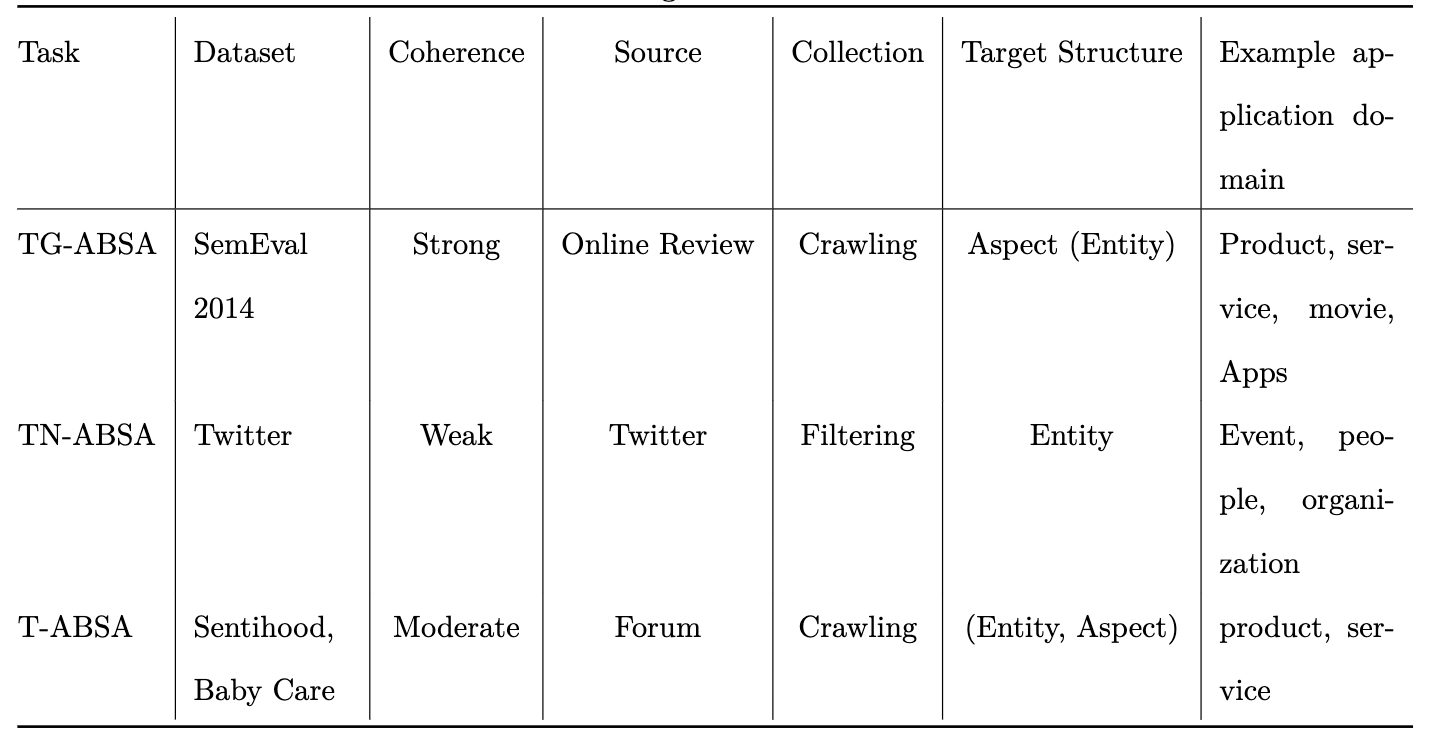
\includegraphics[width=0.7\linewidth]{./image/task.png}
    \caption{Different Task of Sentiment Analysis}
  \label{example}
\end{figure}

\end{frame}

\subsection{Aspect Based Sentiment Analysis}
\begin{frame}{Aspect Based Sentiment Analysis}{Subtask of ABSA}
  \begin{enumerate}
    \item Subtask 1:Aspect term extraction
    \item Subtask 2:Aspect term polarity
    \item Subtask 3:Aspect category detection
    \item Subtask 4:Aspect category polarity
  \end{enumerate}

  The subtask 2, aspect term can be seen as a target, which can be formatted to targeted sentiment analysis.\cite{pontiki-etal-2014-semeval}
\end{frame}


\subsection{Targeted Sentiment Analysis}

\begin{frame}{Targeted Sentiment Analysis}{Task Setting}
  \small
  “I loved their fajitas” → {fajitas: positive}\\
  “I hated their fajitas, but their salads were great” → {fajitas: negative, salads: positive}\\
  “The fajitas are their first plate” → {fajitas: neutral}\\
  “The fajitas were great to taste, but not to see” → {fajitas: conflict}\\
\end{frame}



\begin{frame}{Formal Definition}



\begin{equation}
Sentence=\{w_1,w_2,w_3,w_4,..[t_1,t_2,...,t_m]....,w_n\}
\end{equation}
\begin{equation}
Target \  Text=  \{t_1,t_2,...,t_m\}
\end{equation}
\begin{equation}
polarity=\{positive,neutral,negative\}
\end{equation}

\end{frame}



\section{Related Work}
\subsection{Pre-trained Language Models}

\begin{frame}
\begin{figure}[tp]
  \centering
  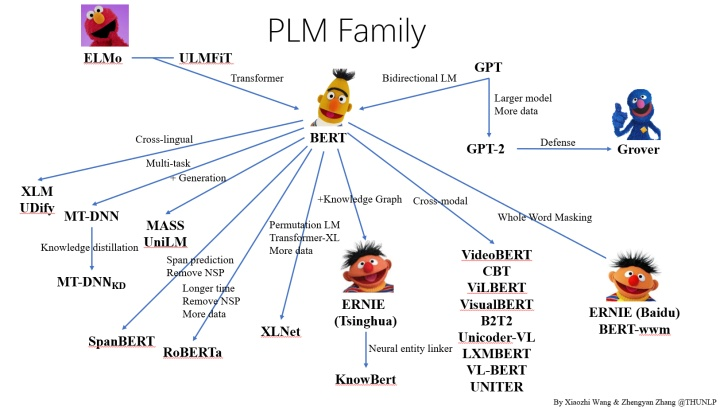
\includegraphics[width=0.7\linewidth]{./image/PLM.jpg}
  \caption{Pre-trained Language Models Family}
\label{example}
\end{figure}

\end{frame}


\subsection{Text Classification}
\begin{frame}{Text Classification}{BERT-Based Methods}
  To utilize bert, we have several direct ways:
  \begin{enumerate}
      \item Using BERT embeddings as the input of a sequence
      \item Fine-tuned BERT by [CLS] classification token.
  \end{enumerate}
  
\end{frame}

\begin{frame}
How to fine-tune BERT for text classification.\cite{sun2019finetune}
  \begin{enumerate}
    \item Various fine tuning methods
    \begin{enumerate}
        \item Within-task pre-training
        \item In-domain pre-training
        \item Cross-domain pre-training
    \end{enumerate}
    
    \item Different learning rates are used for different layers of BERT
\end{enumerate}

\end{frame}


\subsection{Targeted Based Sentiment Analysis}
\begin{frame}

\begin{table}[tp]
  \small
  \centering
  \resizebox{\textwidth}{!}{
  \begin{threeparttable}
  \caption{Previous Work on three typical datasets}
    \begin{tabular}{cccccccc}
    \toprule
    \multirow{2}{*}{ }&\multirow{2}{*}{{Models}}&
    \multicolumn{2}{c}{{Twitter}}&\multicolumn{2}{c}{{Restaurant}}&\multicolumn{2}{c}{{Laptop}}\cr
    \cmidrule(lr){3-4} \cmidrule(lr){5-6} \cmidrule(lr){7-8}
    &&Accuracy&Macro-F1&Accuracy&Macro-F1&Accuracy&Macro-F1\cr
    \midrule
        \multirow{4}*{\textbf{RNN baselines}}
        &TD-LSTM           &0.7080&0.6900              &0.7563&-                  &0.6813&-         \cr
        &ATAE-LSTM         &-&-                        &0.7720&-                  &0.6870&-         \cr
        &IAN               &-&-                        &0.7860&-                  &0.7210&-         \cr
        &RAM               &0.6936&0.6730              &0.8023&0.7080             &{0.7449}&{0.7135}     \cr
    \midrule
        \multirow{3}*{\textbf{Non-RNN baselines}}
        &Feature-based SVM &0.6340&0.6330              &0.8016&-                  &0.7049&-           \cr
        &Rec-NN            &0.6630&0.6590              &-&-                       &-&-              \cr
        &MemNet            &0.6850&0.6691              &0.7816&0.6583             &0.7033&0.6409    \cr

    \midrule
        \multirow{3}*{\textbf{AEN-BERT}}
        &AEN-GloVe  &{0.7283}&0.6981  &{0.8098}&{0.7214}  &0.7351&0.6904 \cr
        &BERT-SPC  &{0.7355}&{0.7214} &{0.8446}&{0.7698} &{0.7899}&{0.7503} \cr
        &AEN-BERT &{0.7471}&{0.7313} &{0.8312}&{0.7376} &{0.7993}&{0.7631} \cr
    \bottomrule
    \end{tabular}
    \label{tab:result}
    \end{threeparttable}}
\end{table}

\end{frame}


\subsection{Previous Work Problems}
\begin{frame}{Previous Work Problems}
\begin{enumerate}
  \item Modeling the data from different aspects, which makes the model not general enough for further improvements.
  \item Targeted-Dependent
  
\end{enumerate}
\end{frame}



% Placing a * after \section means it will not show in the
% outline or table of contents.
\section{Robust Framework}
\subsection{Framework}

\begin{frame}{Framework}
\begin{figure}[h]
  \centering
  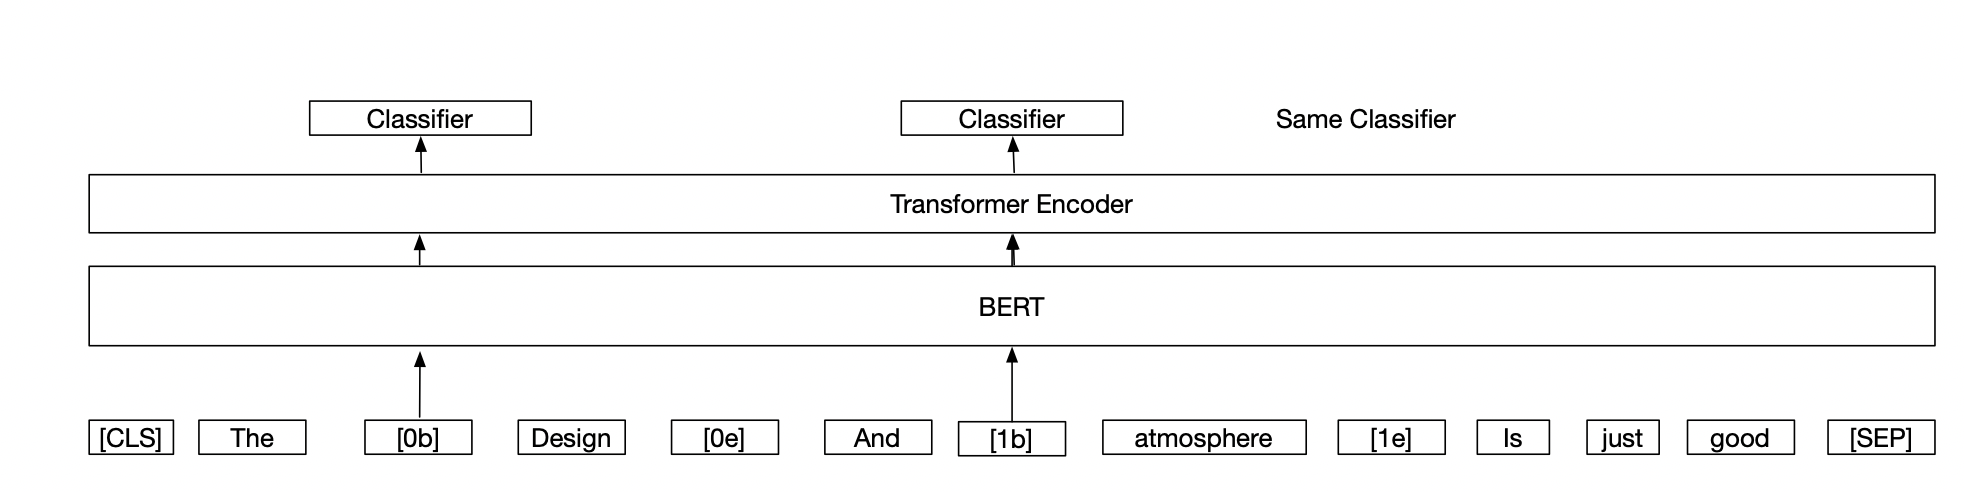
\includegraphics[width=\linewidth]{./image/Framework.png}
  \caption{Our framework for TSA}
\label{Framework}
\end{figure}
\end{frame}

\subsection{Auxiliary Training}
\begin{frame}{Auxiliary Training}
\begin{figure}[h]
  \centering
  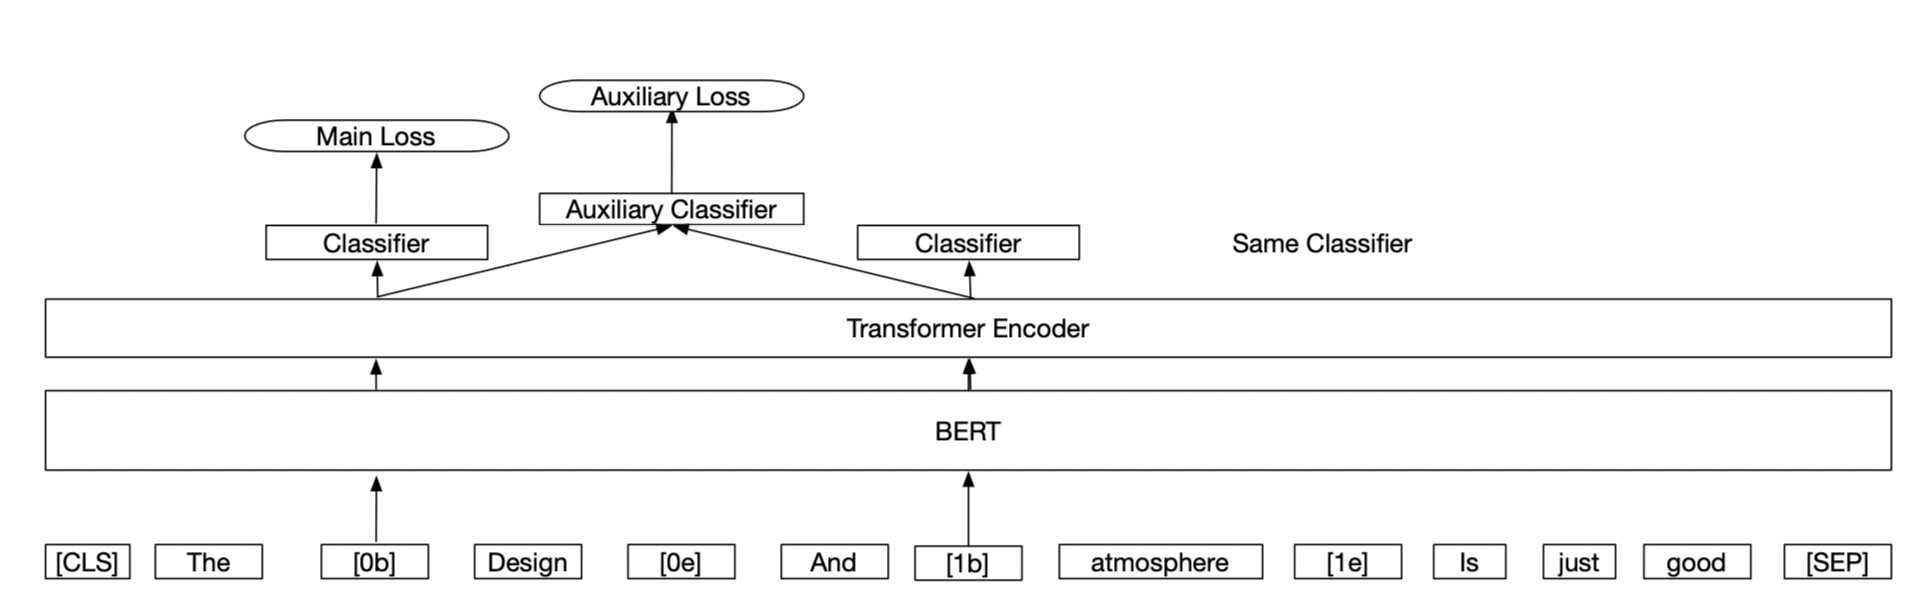
\includegraphics[width=\linewidth]{./image/aux.png}
  \caption{auxiliary training}
\label{Framework}
\end{figure}
\end{frame}

\subsection{Robust Test}
\begin{frame}{Visualization}
  There BERT may have some dependency on the target tokens.
  \begin{figure}[h]
    \centering
    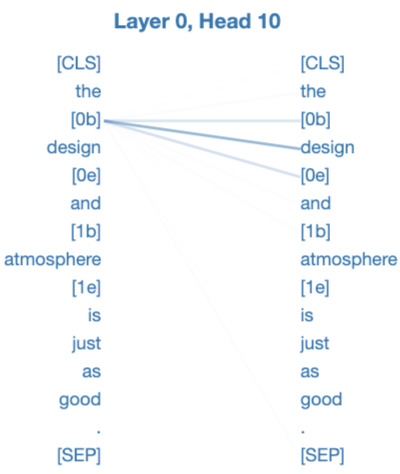
\includegraphics[width=0.3\linewidth]{./image/target-depence.png}
    \caption{visualization of the BERT Bottom layer }
  \label{target-depence}
\end{figure}
\end{frame}

\begin{frame}{Robust Test}
For explicitly test the robustness of model towards unseen target, we proposed the robustness dataset.
\begin{enumerate}
  \item Removing the test samples with the same or similar target in training set.
  \item Re-split the data set.
\end{enumerate}


\end{frame}


\subsection{Adversarial Training}
\begin{frame}{Adversarial Training}
\begin{equation}
r_{adv} = -\epsilon \frac{g}{||g||_2}
\end{equation} 

\begin{equation}
    g = \nabla_{x}\, \log\,  p(y|x;\hat{\theta})
\end{equation} and $p_{adv}=\epsilon$ is the size of the perturbations.

\begin{equation}
	loss_{aux}=- \log p(y|x + r_{adv};\theta)
\end{equation}
The total training loss is:  
\begin{equation}
  \small
    loss(main\ target)=loss_{main}(begin\_{token})+p_{aux}*loss_{aux}(main\ target)+loss_{adv}
\end{equation}

\end{frame}


\subsection{Data Augmentation}
\begin{frame}{Data Augmentation}
Replace the target words using wordnet synonyms.

$augment(target \ words)=synonyms$


For example: \\

augment('laptop')='laptop computer'


augment('staff')='faculty'
\end{frame}


\section{Experiment}
% \subsection{Datasets}
\subsection{TSA Results}

\begin{frame}
\begin{table}
  \small
  \centering
  \resizebox{\textwidth}{!}{
  \begin{threeparttable}
  \caption{
  Test results on three typical data sets.
}
    \begin{tabular}{cccccccc}
    \toprule
    \multirow{2}{*}{ }&\multirow{2}{*}{\ {Models}}&
    \multicolumn{2}{c}{\ {Twitter}}&\multicolumn{2}{c}{\ {Restaurant}}&\multicolumn{2}{c}{\ {Laptop}}\cr
    \cmidrule(lr){3-4} \cmidrule(lr){5-6} \cmidrule(lr){7-8}
    &&Accuracy&Macro-F1&Accuracy&Macro-F1&Accuracy&Macro-F1\cr
    \midrule
        \multirow{4}*{\ {RNN baselines}}
        &TD-LSTM           &0.7080&0.6900              &0.7563&-                  &0.6813&-         \cr
        &ATAE-LSTM         &-&-                        &0.7720&-                  &0.6870&-         \cr
        &IAN               &-&-                        &0.7860&-                  &0.7210&-         \cr
        &RAM               &0.6936&0.6730              &0.8023&0.7080             &\ {0.7449}&\ {0.7135}     \cr
    \midrule
        \multirow{3}*{\ {Non-RNN baselines}}
        &Feature-based SVM &0.6340&0.6330              &0.8016&-                  &0.7049&-           \cr
        &Rec-NN            &0.6630&0.6590              &-&-                       &-&-              \cr
        &MemNet            &0.6850&0.6691              &0.7816&0.6583             &0.7033&0.6409    \cr
    \midrule
        \multirow{3}*{\ {AEN-BERT}}
      %   &AEN-GloVe  &\ {0.7283}&0.6981  &\ {0.8098}&\ {0.7214}  &0.7351&0.6904 \cr
          &BERT &0.7464&0.7304 & 0.8128 & 0.6979 & 0.7654 & 0.7283\\
          &BERT-SPC  &\ {0.7355}&\ {0.7214} &\ {0.8446}&\ {0.7698} &\ {0.7899}&\ {0.7503} \cr
        &AEN-BERT &\ {0.7471}&\ {0.7313} &\ {0.8312}&\ {0.7376} &\ {0.7993}&\ {0.7631} \cr
  \midrule
      \multirow{1}*{\ {BERT-PT}}
      &BERT-PT  &-&-  &\ {0.8495}&\ {0.7696}  &0.7807&0.7508 \cr
  \midrule
      \multirow{2}*{\ {TD-BERT}}
      &TD-BERT  &0.7669&0.7428  &\ {0.8510}&\ {0.7835}  &0.7807&0.7508 \cr
      
      &TD-BERT-QA-CON  & 0.7731&0.7440  &{0.8456}&{0.7961}  &0.7842&0.7437 \cr

  \midrule
      \multirow{2}*{\ {Our}}
      &Framework  &0.7673&0.7451  &\ {0.843}&\ {0.780}  &
      0.7633&0.7291 \cr
      &Framework+aux1.0  &-&-  &\textbf{0.8554}&\textbf{0.7962}  &\textbf{0.7806}&\textbf{0.7523} \cr
      &Framework+aux0.1  &-&-  &\ {0.8464}&\ {0.788}  &0.7759&0.7370 \cr


    \bottomrule
    \end{tabular}
    \label{tab:result}
    \end{threeparttable}}
\end{table}

\end{frame}


\subsection{Domain Adaption Results}

\begin{frame}
  \begin{table}
    \centering
    \tiny
    \caption{Test results on three domain bert}
    \label{domain-res} 



    \begin{tabular}{llllllll}
    \hline
           &           & Twitter &        & Restaurant &         & Laptop &        \\ \hline
    Domain & Method    & acc      & f1     & acc         & f1      & acc    & f1     \\ \hline

    % \midrule
    % \multirow{3}*{\ {BERT-ADA}}
    joint&BERT-ADA Joint  &{-}&{-} &{0.8635}&{0.7889} &{0.7896}&{0.7418} \\ \hline
    rest&BERT-ADA Rest  &{-}&{-} &{0.8714}&{0.8005} &{0.7860}&{0.7409}\\ \hline
    lapt&BERT-ADA Lapt  &{-}&{-} &{0.8551}&{0.7809}&{0.7919}&{0.7418} \\ \hline
    \midrule
           & Framework & 0.7673   & 0.7451 & 0.843       & 0.7808  & 0.7633 & 0.7291 \\ \hline
           & aux 1     & -        & -      & 0.8554      & 0.7962  & 0.7806 & 0.7523 \\ \hline
           & aux 0.1   & -        & -      & 0.8464      & 0.7883  & 0.7759 & 0.737  \\ \hline
    joint  & Framework & -        & -      & 0.8491      & 0.7697  & 0.7821 & 0.7421 \\ \hline
           & aux 1     & -        & -      & 0.8768      & 0.8153  & 0.7978 & 0.7506 \\ \hline
           & aux 0.1   & -        & -      & 0.8625      & 0.8017  & 0.7915 & 0.745  \\ \hline
           rest    & Framework & -        & -      & 0.86911     & 0.8061  & 0.7931 & 0.7461 \\ \hline
           & aux 1     & -        & -      & 0.8786      & 0.8139  & 0.7978 & 0.7571 \\ \hline
           & aux 0.1   & -        & -      & 0.87589     & 0.81696 & 0.7978 & 0.7538 \\ \hline
    lapt    & Framework & -        & -      & 0.8562      & 0.7928  & 0.79   & 0.7477 \\ \hline
           & aux 1     & -        & -      & 0.8786      & 0.8139  & 0.8088 & 0.7627 \\ \hline
           & aux 0.1   & -        & -      & 0.87589     & \textbf{0.81696} & 0.8025 & \textbf{0.7653} \\ \hline
    \end{tabular}
    \end{table}
  \end{frame}


\subsection{Robust Test Results}

\begin{frame}{Rmoving the Test samples with seen targets}
  
  For simplicity, we remove those test samples with the same or similar targets in the training set.



\begin{table}[]
  \centering
  \caption{Statistics of re-split dataset.}
  \begin{tabular}{llll}
  \hline
  dataset  & stat-type         & train & test \\ \hline
  twitter    & size          & 6248 & 619 \\ \hline
             & target-number & 104  & 358 \\ \hline
  restaurant & size          & 3608 & 393 \\ \hline
             & target-number & 606  & 304 \\ \hline
  laptop     & size          & 2328 & 282 \\ \hline
             & target-number & 461  & 232 \\ \hline
  \end{tabular}
\end{table}

\end{frame}

\begin{frame}
  \begin{table}
    \small
    \centering
    \resizebox{\textwidth}{!}{
    \begin{threeparttable}
    \caption{
		Test results on three re-split(removing) data sets.
		% The baselines results are from the existed paper's reports. \\
		% '-' means do not include included in the original paper or the test can not be done in this data set. 
		% The highest score is marked with \ {bold}.
	}
      \begin{tabular}{cccccccc}
      \toprule
      \multirow{2}{*}{ }&\multirow{2}{*}{\ {Models}}&
      \multicolumn{2}{c}{\ {Twitter}}&\multicolumn{2}{c}{\ {Restaurant}}&\multicolumn{2}{c}{\ {Laptop}}\cr
      \cmidrule(lr){3-4} \cmidrule(lr){5-6} \cmidrule(lr){7-8}
      &&Accuracy&Macro-F1&Accuracy&Macro-F1&Accuracy&Macro-F1\cr
      
      

      \midrule
          \multirow{1}*{\ {}}
          &BERT-SPC  &\ {0.7052}&\ {0.6898} &\ {0.7857}&\ {0.6570} &\ {0.7524}&\ {0.6875} \cr



    \midrule
        \multirow{2}*{\ {Our}}
        &Framework  &0.7197&0.7054  &0.8420&0.7740  &0.7696& 0.7282 \cr
        &Framework+adv1 &0.7673&0.7513  &0.8545& \textbf{0.7954}  &0.7821&0.7420 \cr
        &Framework+aux1 &-&-  &0.8420& 0.7735  &0.7774&0.7466 \cr
        &Framework+adv1+aux1 &-&-  &0.8500& 0.7742  &0.7884& \textbf{0.7466} \cr
      \bottomrule
      \end{tabular}
      \label{tab:result}
      \end{threeparttable}}
  \end{table}
\end{frame}


\begin{frame}{Resplit the Datasets}

For comparable to original datasets, we combine the training set and test set together. Then we re-split the datasets by the target.

\begin{table}[]
  \centering
  \tiny
  \caption{Test Results on the re-split datasets}
  \label{tab:my-table}
  \begin{tabular}{llllllll}
    \toprule
  Model   &Methods& Twitters &        & Restaurants &        & Laptops &        \\
  \midrule

            &               & acc      & f1     & acc         & f1     & acc     & f1     \\
  BERT-SPC  & BERT-SPC      & 0.6162   & 0.6132 & 0.7551      & 0.6242 & 0.7247  & 0.683  \\
            & aug           & 0.6224   & 0.616  & 0.7645      & 0.6502 & 0.7154  & 0.645  \\
      \midrule

  Framework & Framework     & 0.6702   & 0.6583 & 0.7701      & 0.6426 & 0.736   & 0.7165 \\
            & aug           & 0.6778   & 0.6668 & 0.7757      & 0.6805 & 0.7566  & 0.7332 \\
            & aux1          &          &        & 0.7888      & \textbf{0.7061} & 0.7453  & 0.7309 \\
            & adv1          & 0.6759   & \textbf{0.6709}& 0.7925      & 0.6773 & 0.7566  & 0.7334 \\
            & aug+adv1      & 0.6479   & 0.6293 & 0.7888      & 0.6881 & {0.7753}  & \textbf{0.7574} \\
            & aux1+adv1     &          &        & 0.7664      & 0.6809 & 0.7528  & 0.7318 \\
            & aug+aux1+adv1 &          &        & 0.7477      & 0.643  & 0.7303  & 0.7158\\
            \bottomrule
  \end{tabular}
  \end{table}

\end{frame}


\section{Conclusion And Future Work}
\begin{frame}{Conclusion}
  \begin{enumerate}
    \item We propose a general framework and auxiliary training method for targeted sentiment analysis. Our results on TSA task is reach or achieve better performance on original datasets.
    \item We propose a robust test dataset for unseen targets.
    \item Our framework is less target-dependent and more robust towards unseen targets.
    \item We implemented two methods to enhance the robustness based on our framework.

  \end{enumerate}
\end{frame}

\begin{frame}{Future Work}
  \begin{enumerate}
    \item 
    {
     Try to combine three methods for robustness.
    }
    \item 
    {
      Data Augmentation for auxiliary training.
    }
  \end{enumerate}
\end{frame}
% Bibliography section. Use \bibitem to add more bibliography items.
\section*{Reference}
\tiny
\nocite{*}
\begin{frame}[allowframebreaks]{Reference}
\bibliography{slides}
\bibliographystyle{unsrt}


\end{frame}

\end{document}